\documentclass{beamer}\usepackage[]{graphicx}\usepackage[]{color}
%% maxwidth is the original width if it is less than linewidth
%% otherwise use linewidth (to make sure the graphics do not exceed the margin)
\makeatletter
\def\maxwidth{ %
  \ifdim\Gin@nat@width>\linewidth
    \linewidth
  \else
    \Gin@nat@width
  \fi
}
\makeatother

\definecolor{fgcolor}{rgb}{1, 0.894, 0.769}
\newcommand{\hlnum}[1]{\textcolor[rgb]{0.824,0.412,0.118}{#1}}%
\newcommand{\hlstr}[1]{\textcolor[rgb]{1,0.894,0.71}{#1}}%
\newcommand{\hlcom}[1]{\textcolor[rgb]{0.824,0.706,0.549}{#1}}%
\newcommand{\hlopt}[1]{\textcolor[rgb]{1,0.894,0.769}{#1}}%
\newcommand{\hlstd}[1]{\textcolor[rgb]{1,0.894,0.769}{#1}}%
\newcommand{\hlkwa}[1]{\textcolor[rgb]{0.941,0.902,0.549}{#1}}%
\newcommand{\hlkwb}[1]{\textcolor[rgb]{0.804,0.776,0.451}{#1}}%
\newcommand{\hlkwc}[1]{\textcolor[rgb]{0.78,0.941,0.545}{#1}}%
\newcommand{\hlkwd}[1]{\textcolor[rgb]{1,0.78,0.769}{#1}}%
\let\hlipl\hlkwb

\usepackage{framed}
\makeatletter
\newenvironment{kframe}{%
 \def\at@end@of@kframe{}%
 \ifinner\ifhmode%
  \def\at@end@of@kframe{\end{minipage}}%
  \begin{minipage}{\columnwidth}%
 \fi\fi%
 \def\FrameCommand##1{\hskip\@totalleftmargin \hskip-\fboxsep
 \colorbox{shadecolor}{##1}\hskip-\fboxsep
     % There is no \\@totalrightmargin, so:
     \hskip-\linewidth \hskip-\@totalleftmargin \hskip\columnwidth}%
 \MakeFramed {\advance\hsize-\width
   \@totalleftmargin\z@ \linewidth\hsize
   \@setminipage}}%
 {\par\unskip\endMakeFramed%
 \at@end@of@kframe}
\makeatother

\definecolor{shadecolor}{rgb}{.97, .97, .97}
\definecolor{messagecolor}{rgb}{0, 0, 0}
\definecolor{warningcolor}{rgb}{1, 0, 1}
\definecolor{errorcolor}{rgb}{1, 0, 0}
\newenvironment{knitrout}{}{} % an empty environment to be redefined in TeX

\usepackage{alltt}
\usepackage{../371g-slides}
% Uncomment these lines to print notes pages
% \pgfpagesuselayout{4 on 1}[letterpaper,border shrink=5mm,landscape]
% \setbeameroption{show only notes}
\title{Probability review 1}
\subtitle{Lecture 3}
\author{STA 371G}
\IfFileExists{upquote.sty}{\usepackage{upquote}}{}
\begin{document}



\frame{\maketitle}


%%%%%%% Slides start here %%%%%%%

\begin{darkframes}


\begin{frame}{Announcements}
\begin{itemize}[<+->]
  \item Homework 1 due Sunday night at 11:59 PM
  \item First (optional) R help session will be this Friday from 11 AM to 12 PM in GSB 3.138 (note temporary room change)
  \item About grading
   \begin{itemize}
     \item QUEST: two tries on each question for full credit, then decreasing credit for each subsequent try
     \item Learning Catalytics: answer 75\% of in-class questions for full participation credit
   \end{itemize}
\end{itemize}
\end{frame}

\begin{frame}
\begin{center}
  What are the chances that two people \emph{in this room} have the same birthday (month/day, not year)?
  \lc
\end{center}
\end{frame}

\begin{frame}{Probability Theory}
\framesubtitle{The Concept of Probability}

What do each of these have in common? \pause

\begin{itemize}[<+->]
	\item Outcome of rolling a die
	\item S\&P500 index at the and of January
	\item Number of iPhone 7s to be sold over the next year
	\item Number of unique visitors to Amazon.com over the next week
	\item Lifetime of your MacBook Air
\end{itemize} \pause

We cannot predict any of these with certainty. \pause
But we can model them using \alert{probability theory} and learn a lot about how these variables will behave.
\end{frame}

\begin{frame}{Probability Theory}
\framesubtitle{Definitions}
\begin{definition}
		A \alert{random variable} expresses the outcome of a random process as a number. It is denoted by an uppercase letter.
\end{definition} 	\pause

\begin{itemize}[<+->]
	\item Random experiment $\rightarrow$ Selecting a student at random from the class
	\item Random variable $\rightarrow$ $X:$ The day of their birthday ($1,2,\ldots,31$)
  \item Random variable $\rightarrow$ $Y:$ Their height, in inches
\end{itemize}
\end{frame}


\begin{frame}{Probability Theory}
\framesubtitle{Definitions}

\begin{definition}
		A \alert{discrete random variable} is a random variable with a finite (or countably infinite) range.  \pause

		A \alert{continuous random variable} is a random variable with an interval (either finite or infinite) of real numbers for its range.
\end{definition} \pause

\begin{itemize}[<+->]
  \item $X:$ Number of stocks on NYSE whose price change today (discrete)
  \item $Y:$ Average price change of the stocks on NYSE (continuous)
  \item $Z:$ Number of people that lose money in the stock market today (discrete!)
\end{itemize}
\end{frame}


\begin{frame}{Probability Theory}
\framesubtitle{Exercise}
Discrete or continuous?  \pause
\begin{itemize}[<+->]
	\item Number of iPhone 7s to be sold over the next year  \pause (discrete)
	\item Lifetime of your MacBook Air, in years  \pause (continuous)
	\item Number of unique visitors to Amazon.com over the next week  \pause (discrete)
  \item S\&P 500 index at the and of January \pause (continuous)
\end{itemize}
\lc
\end{frame}


\begin{frame}{Probability Theory}
\framesubtitle{Definitions}
\begin{definition}
	\alert{Probability} is the measure of the likelihood that a particular outcome (or set of outcomes) will be observed. Probability is a number always between 0 and 1.
\end{definition} \pause

\begin{itemize}[<+->]
  \item $X:$ The month number of the student's birthday, $P(X=3)=1/12$
	\item $Y:$ Lifetime of your MacBook, $ P(Y>5\text{ years})  = 0.05$
\end{itemize}
\end{frame}


\begin{frame}{Probability Distributions}
Now that we have defined a random variable, how do we know what the probabilities are? \newline \pause

For example, what is the probability that your MacBook will break down after 5 years but before 7 years? That is, $P(5<X<7)=?$\newline \pause

\begin{definition}
	The \alert{probability distribution} of a random variable $X$ is a description of the probabilities associated with the possible values of $X$. \newline \pause
	Discrete random variable $\rightarrow$ Probability Mass Function (p.m.f.) \pause
	Continuous random variable $\rightarrow$ Probability Density Function (p.d.f.)
\end{definition}
\end{frame}


\begin{frame}{Discrete Random Variables}
  Michael Beuoy's model for NFL games gives the following probabilities for the Super Bowl (positive margin = Patriots win):

  \begin{center}
    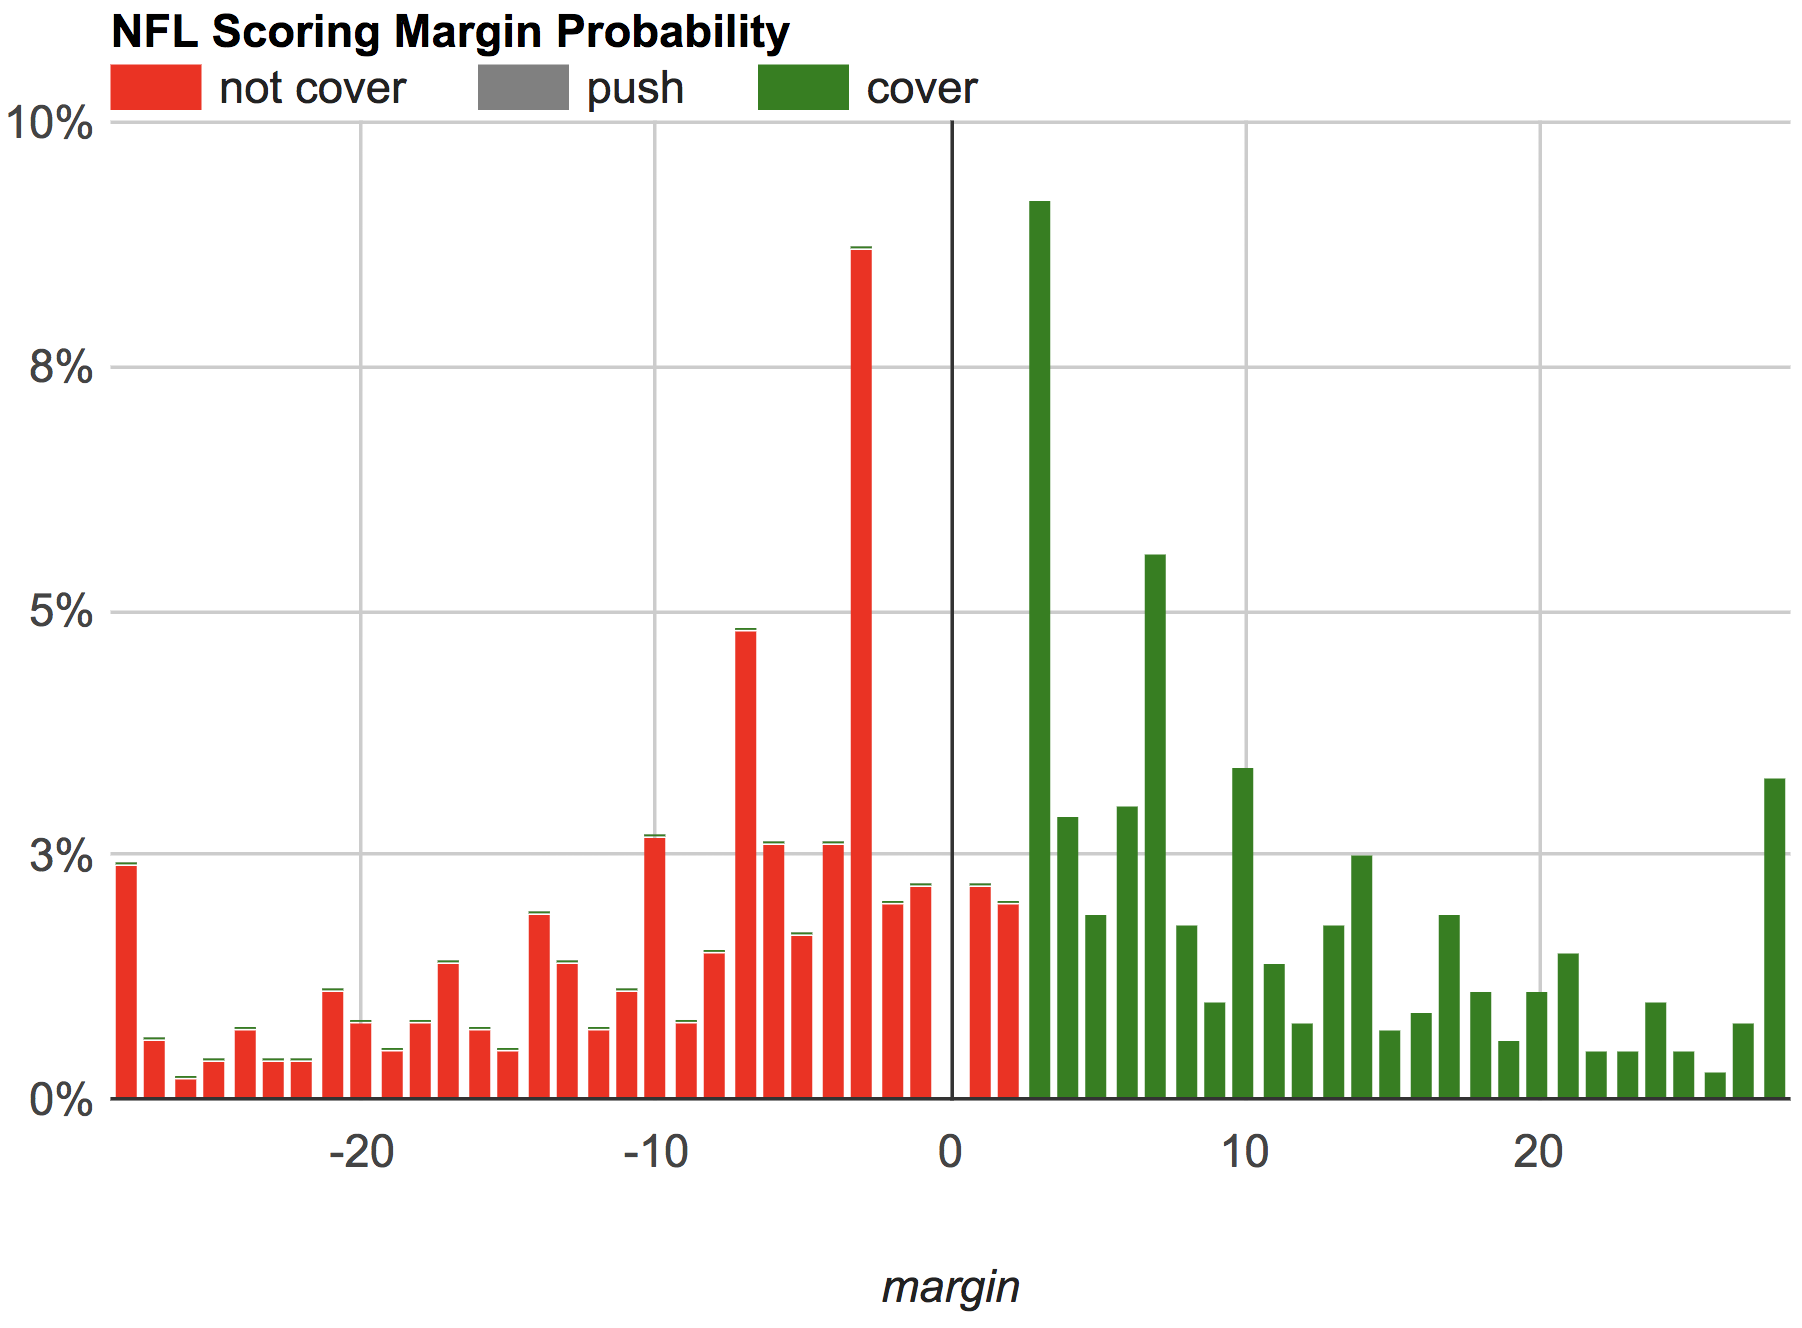
\includegraphics[height=2in]{super-bowl}
  \end{center}
\end{frame}

\begin{frame}[fragile]{Discrete Random Variables}
Let $M$ be a random variable representing the Patriots' margin of victory.
\begin{center}
  \begin{tabular}{cc}
    Patriots' margin of victory & Probability \\
    $m$ & $P(M=m)$ \\
    \hline
    $-28$ & $0.024$ \\
    $-27$ & $0.006$ \\
    $-26$ & $0.002$ \\
    $-25$ & $0.004$ \\
    \vdots & \vdots \\
    $27$ & $0.008$ \\
    $28$ & $0.033$ \\
  \end{tabular}
\end{center}
\end{frame}

\begin{frame}[fragile]{Discrete Random Variables}

\begin{definition}
  The \alert{expected value} and \alert{variance} of a random variable $X$ are the long run mean and variance if we draw values repeatedly from $X$.
\end{definition}

\pause
\begin{align*}
  E(M) &= \sum_{\text{all margins $m$}} m \cdot P(M=m) \\
  &= (-28)(0.024) +
     (-27)(0.006) + \cdots \\
  \text{Var}(M) &= \sum_{\text{all margins $m$}} (m-E(M))^2 \cdot P(M=m) \\
  &= (-28-E(M))^2(0.024) +
     (-27-E(M))^2(0.006) + \cdots \\
\end{align*}
\note{This is way too painful to do by hand! Show how to calculate $E(M)$ in R.}
\note{LC questions 3-6 here}
\end{frame}


\begin{frame}{Normal Distributions (the ``bell curve'')}
The \alert{normal distribution} is a common continuous probability distribution;
we will denote a normal distribution with mean $\mu$ and variance $\sigma^2$ by $N(\mu,\sigma^2)$.
\end{frame}

\begin{frame}{Normal Distributions (the ``bell curve'')}
\fullpagepicture{normal}
\lc
\end{frame}

\begin{frame}{Continous Random Variables}
Let $V$ be a random variable indicating the SAT Verbal score of a randomly selected student in the US.

\[
  P(\text{SAT} > 600) = \pause \int_{600}^{800} P(V = v) \, dv
\]

\pause

\begin{knitrout}
\definecolor{shadecolor}{rgb}{0.137, 0.137, 0.137}
\input{/tmp/figures/unnamed-chunk-3-1.tikz}

\end{knitrout}
\end{frame}

\begin{frame}{Continuous Random Variables}
Let $V$ be a random variable indicating the SAT Verbal score of a randomly selected student in the US.
\[
  P(\text{SAT} = 600) = \pause 0
\]
\begin{knitrout}
\definecolor{shadecolor}{rgb}{0.137, 0.137, 0.137}
\input{/tmp/figures/unnamed-chunk-4-1.tikz}

\end{knitrout}
\end{frame}


\begin{frame}{Continous Random Variables}
The formulas for expected value and variance are the same for continuous random variables, but they involve integrals instead of sums:

\begin{columns}[T,onlytextwidth]
  \column{.5\textwidth}
    \begin{center}
  	Discrete random variable $X$
    \\

  	\begin{align*}
      E(X) &= \sum_x x  P(X=x) \\
      \text{Var}(X) &= \sum_x (x-E(X))^2 P(X=x)
    \end{align*}
    \end{center}

  \column{.5\textwidth}
    \begin{center}
  	Continuous random variable $Y$

    with density function $f(y)$
  	\begin{align*}
	    E(Y) &= \int_y y f(y) \, dy \\
      \text{Var}(Y) &= \int_y (y-E(Y))^2 f(y)
    \end{align*}
    \end{center}
\end{columns}
\lc
\end{frame}


\begin{frame}[fragile]{R Simulation of expected value}
\framesubtitle{R Simulation}

Let's simulate rolling dice and see that the expected value really does represent the long-run average!

\begin{knitrout}
\definecolor{shadecolor}{rgb}{0.137, 0.137, 0.137}\begin{kframe}
\begin{alltt}
\hlcom{# Simulate rolling a die 1 time}
\hlkwd{sample}\hlstd{(}\hlkwd{c}\hlstd{(}\hlnum{1}\hlstd{,} \hlnum{2}\hlstd{,} \hlnum{3}\hlstd{,} \hlnum{4}\hlstd{,} \hlnum{5}\hlstd{,} \hlnum{6}\hlstd{),} \hlnum{1}\hlstd{,} \hlkwc{replace}\hlstd{=T)}
\hlcom{# Simulate rolling a die 4 times}
\hlkwd{sample}\hlstd{(}\hlkwd{c}\hlstd{(}\hlnum{1}\hlstd{,} \hlnum{2}\hlstd{,} \hlnum{3}\hlstd{,} \hlnum{4}\hlstd{,} \hlnum{5}\hlstd{,} \hlnum{6}\hlstd{),} \hlnum{4}\hlstd{,} \hlkwc{replace}\hlstd{=T)}
\hlcom{# Take the average}
\hlkwd{mean}\hlstd{(}\hlkwd{sample}\hlstd{(}\hlkwd{c}\hlstd{(}\hlnum{1}\hlstd{,} \hlnum{2}\hlstd{,} \hlnum{3}\hlstd{,} \hlnum{4}\hlstd{,} \hlnum{5}\hlstd{,} \hlnum{6}\hlstd{),} \hlnum{4}\hlstd{,} \hlkwc{replace}\hlstd{=T))}
\hlcom{# Let's increase the number of dice}
\hlkwd{mean}\hlstd{(}\hlkwd{sample}\hlstd{(}\hlkwd{c}\hlstd{(}\hlnum{1}\hlstd{,} \hlnum{2}\hlstd{,} \hlnum{3}\hlstd{,} \hlnum{4}\hlstd{,} \hlnum{5}\hlstd{,} \hlnum{6}\hlstd{),} \hlnum{100}\hlstd{,} \hlkwc{replace}\hlstd{=T))}
\end{alltt}
\end{kframe}
\end{knitrout}
\end{frame}


\begin{frame}{Joint probability -- back to birthdays}
If two events are \emph{independent} (i.e., knowing the outcome of one tells you nothing about the outcome of the other), then the probability of two events happening at the same time is
\[ P(\text{$A$ and $B$}) = P(A)P(B). \]
\pause
Let's figure out the probability of no one sharing a birthday. Let's call $B_1$ the first person's birthday, $B_2$ the second person's birthday, etc.
\pause
\begin{align*}
P(\text{none shared}) &= P(B_2 \neq B_1) \cdot P(B_3 \neq B_1,B_2) \cdot P(B_4 \neq B_1,B_2,B_3)\cdots \\
&= \frac{364}{365} \cdot \frac{363}{365} \cdot \frac{362}{365} \cdots
\end{align*}
\pause
When $n=70$ the probability of no shared birthdays is just 0.01\%!
\end{frame}

\end{darkframes}
\end{document}
